\documentclass[onecolumn, draftclsnofoot, 10pt, compsoc]{IEEEtran}
\usepackage{graphicx}
\usepackage{url}
\usepackage{setspace}
\usepackage{listings}
\usepackage{xcolor}

\definecolor{codegreen}{rgb}{0,0.6,0}
\definecolor{codegray}{rgb}{0.5,0.5,0.5}
\definecolor{codepurple}{rgb}{0.58,0,0.82}
\definecolor{backcolour}{rgb}{0.95,0.95,0.92}

\lstdefinestyle{mystyle}{
    backgroundcolor=\color{backcolour},   
    commentstyle=\color{codegreen},
    keywordstyle=\color{magenta},
    numberstyle=\tiny\color{codegray},
    stringstyle=\color{codepurple},
    basicstyle=\ttfamily\footnotesize,
    breakatwhitespace=false,         
    breaklines=true,                 
    captionpos=b,                    
    keepspaces=true,                 
    numbers=left,                    
    numbersep=5pt,                  
    showspaces=false,                
    showstringspaces=false,
    showtabs=false,                  
    tabsize=2
}
\lstset{style=mystyle}

\usepackage{geometry}

\geometry{textheight=9.5in, textwidth=7in}

\usepackage{biblatex}
\addbibresource{references.bib}

\newcommand\ytl[2]{
\parbox[b]{8em}{\hfill{\color{cyan}\bfseries\sffamily #1}~$\cdots\cdots$~}\makebox[0pt][c]{$\bullet$}\vrule\quad \parbox[c]{4.5cm}{\vspace{7pt}\color{red!40!black!80}\raggedright\sffamily #2.\\[7pt]}\\[-3pt]}

% 1. Fill in these details
\def \CapstoneTeamName{Team 42}
\def \CapstoneTeamNumber{		42}
\def \GroupMemberOne{			Michael Burton}
\def \GroupMemberTwo{			Rajat Kulkarni}
\def \GroupMemberThree{			Logan Saso}
\def \GroupMemberFour{			Miao Zhou}
\def \CapstoneProjectName{		Autonomous RC Car}
%\def \CapstoneSponsorCompany{	}
\def \CapstoneSponsorPerson{	D. Kevin McGrath}

% 2. Uncomment the appropriate line belofw so that the document type works
\def \DocType{	%Requirement Document
				%Requirements Document
				%Technology Review
				%Design Document
				End of Term Report
				}
			
\newcommand{\NameSigPair}[1]{\par
\makebox[2.75in][r]{#1} \hfil 	\makebox[3.25in]{\makebox[2.25in]{\hrulefill} \hfill		\makebox[.75in]{\hrulefill}}
\par\vspace{-12pt} \textit{\tiny\noindent
\makebox[2.75in]{} \hfil		\makebox[3.25in]{\makebox[2.25in][r]{Signature} \hfill	\makebox[.75in][r]{Date}}}}
% 3. If the document is not to be signed, uncomment the RENEWcommand below
\renewcommand{\NameSigPair}[1]{#1}

%%%%%%%%%%%%%%%%%%%%%%%%%%%%%%%%%%%%%%%
\begin{document}
\begin{titlepage}
    \pagenumbering{gobble}
    \begin{singlespace}
        \hfill 
        % 4. If you have a logo, use this includegraphics command to put it on the coversheet.
        %\includegraphics[height=4cm]{CompanyLogo}   
        \par\vspace{.2in}
        \centering
        \scshape{
            \huge CS Capstone \DocType \par
            {\large\today}\par
            \vspace{.5in}
            \textbf{\Huge\CapstoneProjectName}\par
            \vfill
            {\large Prepared by }\par
            SmartRC\par
            % 5. comment out the line below this one if you do not wish to name your team
            %\CapstoneTeamName\par 
            \vspace{5pt}
            {\Large
                \NameSigPair{\GroupMemberOne}\par
                \NameSigPair{\GroupMemberTwo}\par
                \NameSigPair{\GroupMemberThree}\par
                \NameSigPair{\GroupMemberFour}\par
            }
            \vspace{20pt}
        }
        \begin{abstract}

        In this document we'll be reviewing the work we've accomplished throughout this quarter and any next steps that we have to accomplish before the April 15th deadline. We'll be going over the project's goals, current status (include what is finished, and what is left to do), as well as a rich selection of code snippets which we'll be going over in-depth.

        \end{abstract}     
    \end{singlespace}
\end{titlepage}
\newpage
\pagenumbering{arabic}
\tableofcontents

\clearpage

\section{Recap}

\subsection{Goals}
The goal of this project is to explore and solve some sub-problems that full-scale autonomous vehicles may encounter. Ideally, it will support plug-able sensors for rapid prototyping of self-driving car models and development of custom solutions. As you'll see in this document, however, we've had some setbacks.

\subsection{Purpose}

The project aims to design and implement an autonomous remote-controlled car that can travel in busy rooms while avoiding collisions with fixed or moving obstacles. Functionally, it should be similar to a large self-driving car.

\section{Current Status}
Despite numerous setbacks, our project is coming along well and we've made significant progress this term. We are currently on track to meet our goals.

\subsection{What's Done}

\subsubsection{Hardware}

For this project we were given an R/C car with an assortment of electrical components, and tasked with creating an autonomous vehicle. This meant that in order for us to implement our solution, we had to fabricate a platform to attach to the R/C car to house the computer and all the sensors. Figure 1 shows all the components we were given to use. 
\begin{figure}[htp]
    \centering
    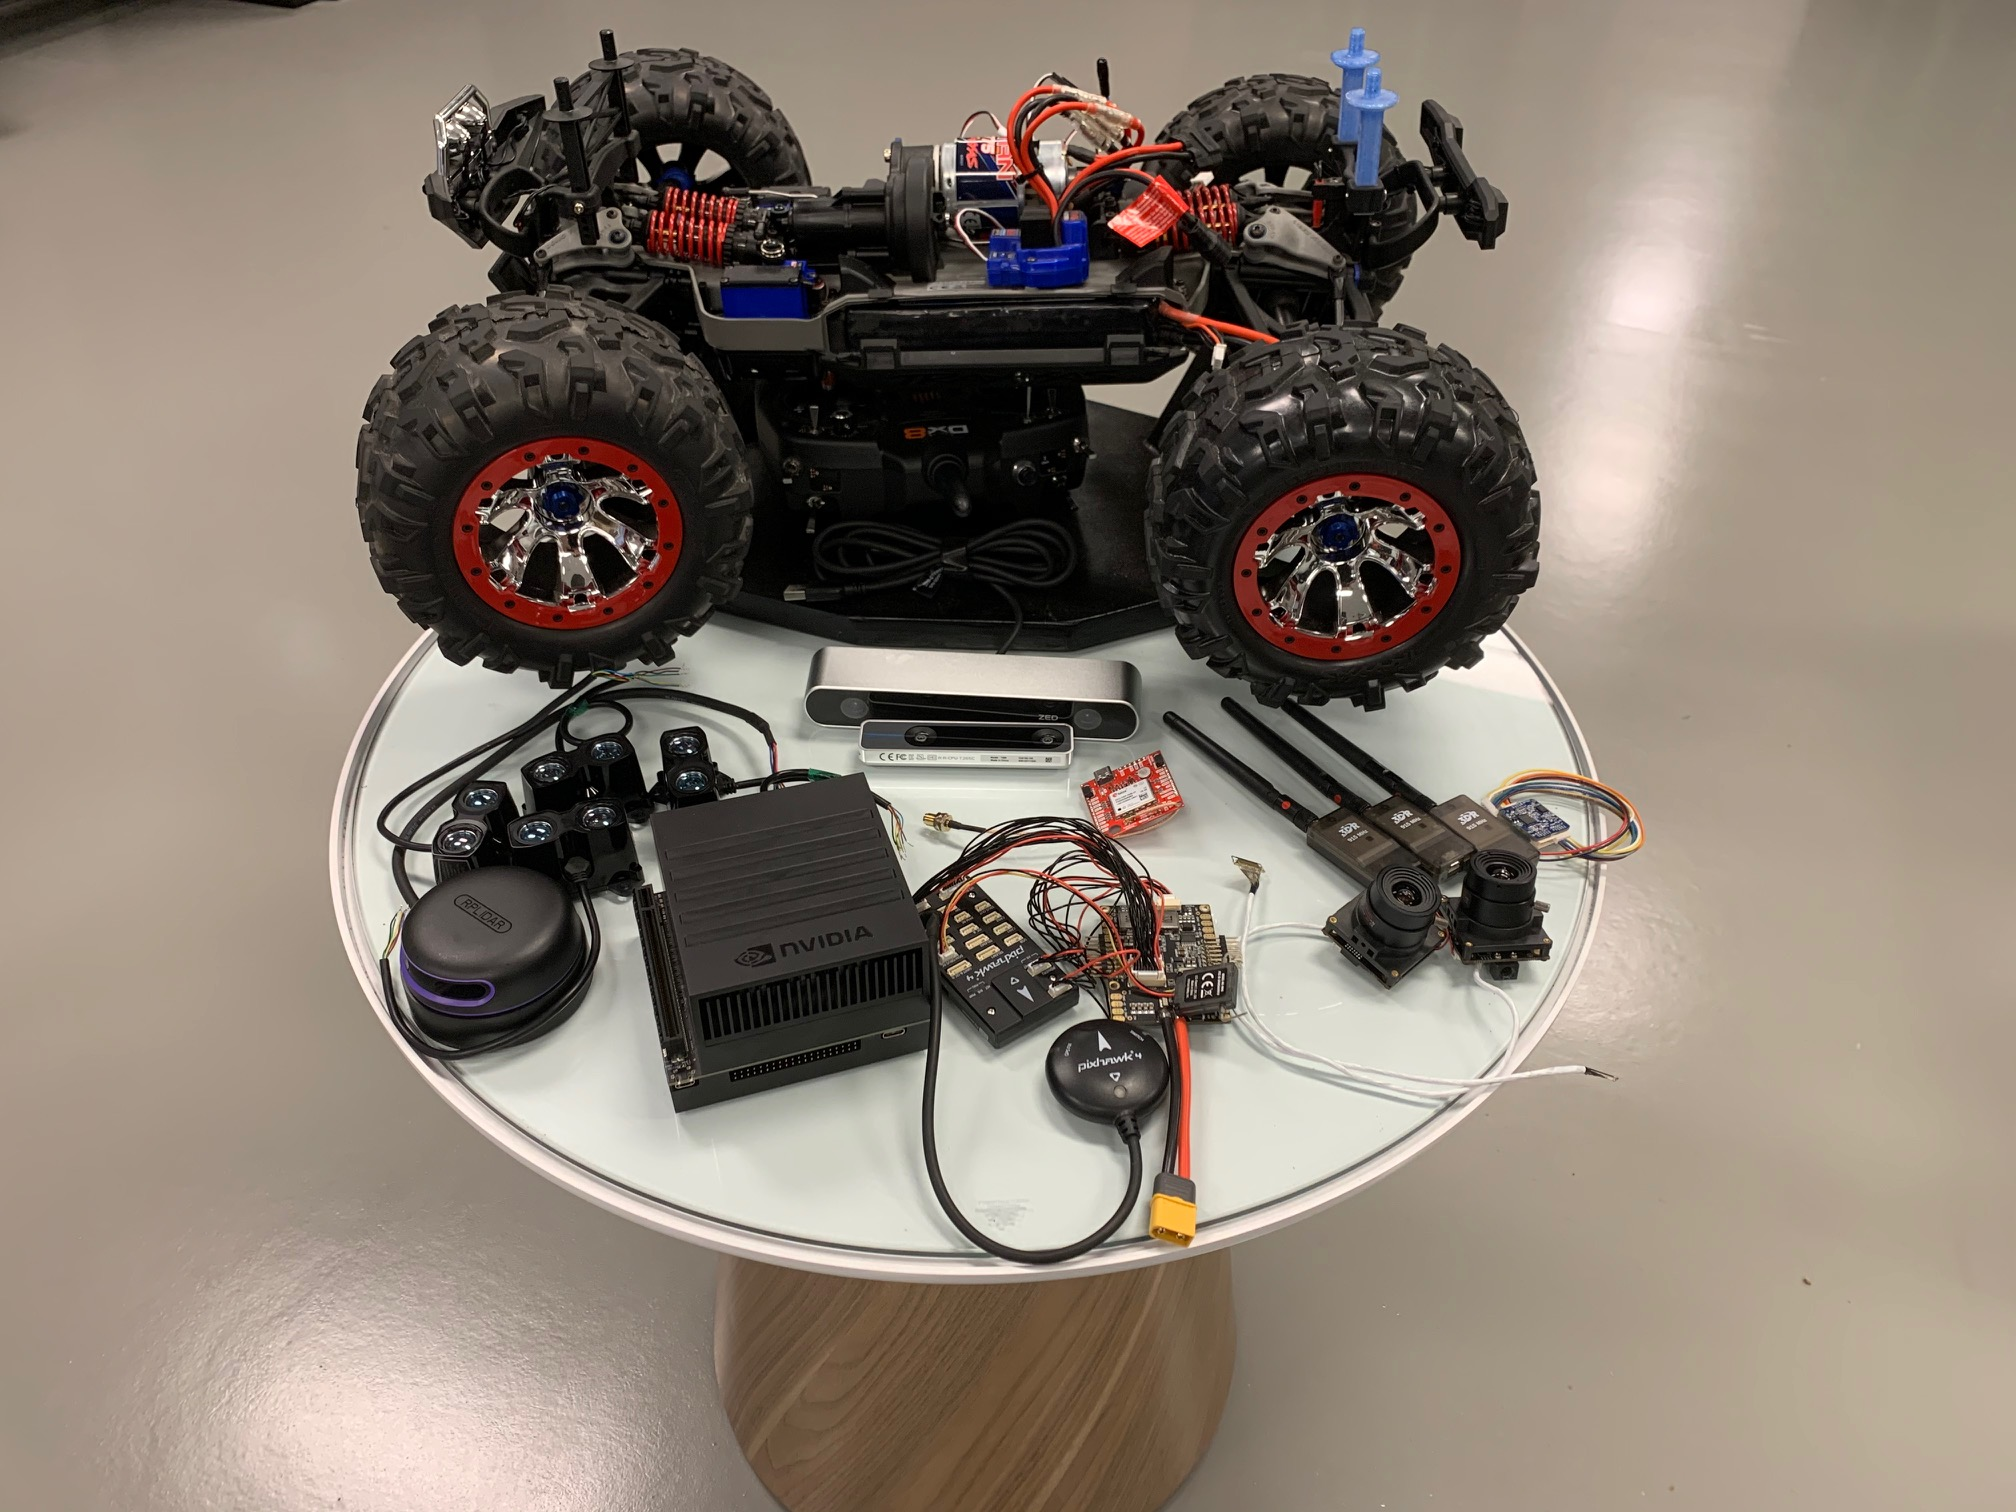
\includegraphics[width=8cm]{given.jpeg}
    \caption{Starting materials given by our client.}
\end{figure}

As detailed in the design document, we had already mapped out the placement for all of the sensors. However, we still needed to build the mounts for them. We obtained a 3/16" sheet of acrylic that we cut to be slightly longer and wider than the car. We did this to provide space for mounts to come down in front of the bumpers and in front of the side of the car. These mounts are for the directional LiDAR sensors. The acrylic sheet is mounted to the car's body through four plastic pegs that stick through the acrylic and are fastened with cotter pins. We then created an aluminum housing for the Nvidia Xavier computer that is mounted to the top of the acrylic. We also created a 3.5" raised platform that has the Slamtec A3 360 LiDAR sensor. We created the raised mount to allow for the sensor to get a full 360 degree view of objects without other components of the car getting in the way.

\begin{figure}[htp]
    \centering
    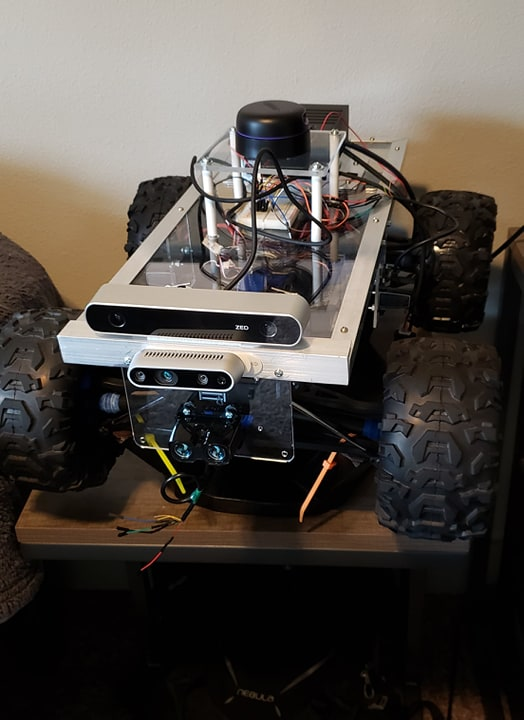
\includegraphics[width=8cm]{Baseplate.jpg}
    \caption{The RC car with all sensors and CPU components mounted.}
\end{figure}

\subsubsection{Software}
On the software side, we've accomplished quite a bit. Through ROS, we have almost entirely set up the Navigation Stack for the robot, which includes a number of components.

One such component is the launch file titled liftoff.launch. This file is essentially the "control center" for the entire set of sensors and ultimately the car. This file contains software for each sensor and their respective transformations.

We've also utilized one of ROS's package, titled "SLAM", to create a 2-dimensional map of the robot's surroundings at any given moment. Although the map isn't updating as frequently as desired, and has some inconsistencies between all the components (such as transformations and sensor data), it still gives a fairly accurate view of the surroundings.

\subsection{What's Left}
\subsubsection{Hardware}
Most of the progress we have left to do remains on the hardware side. One of the biggest issues we've had is getting the motor to function properly. Although everything seems to be wired properly, for reasons we're currently unsure of, we're having trouble getting it to run.
    

\subsubsection{Software}
On the software side, we still need to setup the rest of the navigation stack. Next, and finally, we need to complete creating the move base. The move base package within ROS provides "an implementation of an action that, given a goal in the world, will attempt to reach it with a mobile base"[1]. Since our goal is to provide the robot with certain destinations to travel to, using the move base package is a must.

If time allows, a optional goal is also to implement basic object classification. This would allow the car to view and distinguish between objects - for instance, between a rock and a person. However, this is a reach goal for the team.


\subsection{Problems}
This project has presented us with hardware, software, and logistical challenges.

\subsubsection{Hardware Issues}
We have had numerous issues with wiring the components. We are still dealing with issues in that regard. We ran into multiple problems throughout the term where we would get a piece of hardware that we figured out we needed, only to realize that we needed an additional piece of hardware to make it functional. 

This challenge with hardware has ultimately set us back a good amount. We have also been struggling with getting the car properly wired. We've followed many diagrams, but none have produced a car that is able to move. Unfortunately, none of us are very familiar with this type of work. This gap of knowledge has made it hard to diagnose where we are going wrong. Luckily, we've still been able to implement the software side of making the car move, we just haven't been able to use it yet. This means that once we get the wiring set up correctly we should be good to go. 

\subsubsection{Software Issues}
 
Fortunately, we've had few software issues. However, there have been some issues impeding progress. Namely, there are some strange interactions between sensor data, transformation frames, and the visualization software known as Rviz. Rviz is going to be the main command hub of the project, where we'll see the robot's location in the world map and plot destinations as well as starting points. However, sometimes our RPLidar sensor data reports as not having a valid transformation frame despite being able to see the node in the transformation tree and can see the raw data of the transforms. We're usually able to fix this by restarting Rviz and can continue without problem.

\section{Code Snippets}

\subsection{TF Transforms}

Here we demonstrate an example TF transform. In the final version of our project, we use nothing but static transforms. After writing this code, we discovered that there is a static transforms package which allows us to do the same work, but in the XML configuration which we'll demonstrate later in the code examples. However, it's still useful to see what the code is doing. In the below snippet, we setup a ROS TF publisher. It relates the base\_link frame to the RPLidar laser scan frames. 

This line says, do not rotate, keep position, and associate the frame data as coming in 0.08 meters above the base\_link.

\begin{lstlisting}[language=C++]
b.sendTransform(
	tf::StampedTransform(
		tf::Transform(tf::Quaternion(0, 0, 0, 1), tf::Vector3(0, 0, .08)),
		ros::Time::now(), "base_link", "circle_laser_frame"));
\end{lstlisting}

\subsection{Control Program}

This program lets us send `mavros/manual\_control` messages to the Pixhawk to potentially move the vehicle. It's goal is to use WASD to emulate throttle and direction which might normally be read through a remote controller designed for this device. It loops over standard in, looking for one of WASD and generates a manual control frame based on the input. If the user types anything else, like space, it will just put 0s for everything effectively stopping the vehicle. If the escape key is read (line 15), then the program exits.

\begin{lstlisting}[language=Python]
# imports omitted

dest_node = "/mavros/manual_control/send"
def main():
    print("Starting manual control")
    print("Press WASD to move, hold ESC to exit")
    
    pub = rospy.Publisher(dest_node, ManualControl, queue_size = 1) # Queue size one because we always want the most recent data
    rospy.init_node('manual_control_keyboard')
    rate = rospy.Rate(10) # 10 hz

    frame_id = 0
    while not rospy.is_shutdown():
        ch = read_key()
        if ord(ch) == 27: # If it's the escape key
            exit(1)
        ctrl = get_control(ch, frame_id)
        frame_id += 1
        pub.publish(ctrl)
        rospy.loginfo(ctrl)
        rate.sleep()

def get_control(char, frame_id):
    debugging = False

    multiplier = 0.5
    msg = ManualControl()
    msg.header.frame_id = "manual_control_frame"
    msg.header.seq = frame_id
    now = rospy.get_rostime()
    msg.header.stamp.secs = now.secs
    msg.header.stamp.nsecs = now.nsecs

    if debugging:
        msg.x = multiplier
        msg.y = multiplier
        msg.z = multiplier
        msg.r = multiplier

    if char == 'w':
        msg.x = multiplier * 1

    if char == 's':
        msg.x = multiplier * -1

    if char == 'a':
        msg.y = multiplier * -1

    if char == 'd':
        msg.y = multiplier * 1

    if debugging:
        msg.r = random() % 1 # No roll on car
        msg.z = random() % 1 # No up or down on car
    else:
        msg.r = 0.0
        msg.z = 0.0
    return msg

def read_key():
    fd = sys.stdin.fileno()
    old_settings = termios.tcgetattr(fd)
    try:
        tty.setraw(sys.stdin.fileno())
        ch = sys.stdin.read(1)
    except ValueError:
        exit(1)
    finally:
        termios.tcsetattr(fd, termios.TCSADRAIN, old_settings)
    return ch

if __name__ == "__main__":
    main()
\end{lstlisting}

\subsection{Launch File}

This is where the real meat of the configuration happens. ROS is built of a variety of nodes working together to accomplish a particular goal, whether that is to move a robot, decide on some position, or generate a map of the surrounding areas. Bellow we have broken up our primary launch file which is responsible for starting all of the nodes we use with the Robot. Note that each of the following sections make up only one launch file.

\begin{lstlisting}[language=XML]
<launch>
    <node pkg="rplidar_ros" type="rplidarNode" name="circlelidar" output="screen">
        <param name="serial_port" type="string" value="/dev/ttyUSB0" />
        <param name="serial_baudrate" type="int" value="256000" />
        <param name="frame_id" type="string" value="circle_laser_frame"/>
        <remap from="scan" to="/lidar/scan"/>
    </node>
\end{lstlisting}

This section starts our RPLidar node, and names it `circlelidar` so that it's easy to keep track of. It also is configured to output information to the screen. ROS also allows your nodes to output to log files which you can then look at later, if there are issues. We have to configure a few basic paramters to match what we have on our device, like the serial port. The baudrate is configurable, but we figured a higher baudrate would be better since it allows for more bits to be transferred over the line at once. We also changed the frame id to be `circle\_laser\_frame` so that it is distinct in our node graph. Otherwise, it would simply publish as a `laser\_frame` which is also used by our directional lidar. We also remap the output publisher name from `scan` to `lidar/scan` so that we have a distinct scan publisher for this node. Otherwise, the zed scan would conflict with it.

\begin{lstlisting}[language=XML]
    <node pkg="zed_wrapper" type="zed_wrapper_node" name="zedodom" output="screen">
        <rosparam file="$(find zed_wrapper)/params/common.yaml" command="load"/>
        <rosparam file="$(find zed_wrapper)/params/zed.yaml" command="load"/>

        <param name="camera_name" value="zed"/>
        <param name="camera_model" value="zed"/>
        <param name="general/frame_rate" value="100"/>
        <param name="general/resolution" value="3"/>
        <param name="pos_tracking/odometry_frame" value="zedodom"/>
    </node>
\end{lstlisting}

This section holds the configuration for our ZED stereoscopic camera node, which we named zedodom, and publish to the screen. Unlike the previous section, use some `rosparam` keywords to import basic parameters that come with the zed camera wrapper. Then, we make sure to configure a few of the base parameters so that they never change. For example, we want the highest framerate possible so that we can have the fastest updates and, potentially, avoid obstacles as quickly as possible. We also have opted for resolution 3, which means we want to use VGA-level quality. This is because the ZED camera has a tradeoff in resolution vs speed. To get 100fps, we had to lower the resolution to VGA quality. 3 is the lowest quality with VGA, and it goes up to HD2K (usually around 2000x1000 pixels) at setting 0. Like before, we remap the frame to a custom string so that we can uniquely identify it later in other nodes.

\begin{lstlisting}[language=XML]
    <node pkg="pointcloud_to_laserscan" type="pointcloud_to_laserscan_node" name="zed_pointcloud_to_laserscan" output="screen">
        <remap from="cloud_in" to="/zedodom/point_cloud/cloud_registered"/>
        <remap from="scan" to="/zed/scan"/>
        <param name="scan_time" type="double" value="0.01"/>
    </node>
\end{lstlisting}

This section is responsible for converting the ZED's pointcloud to a laserscan. The node takes any PointCloud2 type and converts it into a LaserScan type, which we can use in our gmapping configuration (below) to generate the map of the world as we move through it. For this, all we had to configure was the PointCloud2 input, the corresponding output (/zed/scan), and the length of the scan to be one one-hundredth of a second (to match our frame rate).

\begin{lstlisting}[language=XML]
    <node pkg="gmapping" type="slam_gmapping" name="slam_provider" output="screen">
        <remap from="scan" to="/lidar/scan"/>
        <param name="map_update_interval" value="0.1"/>
        <param name="linearUpdate" value="0.1"/>
        <param name="angularUpdate" value="0.1"/>
        <param name="particles" value="1"/>
        <param name="delta" value="0.1" />
    </node>
\end{lstlisting}

This section is perhaps the most important, parameter wise. This is where we configure the mapping program which takes in all the information about our laser scans and builds a worldmap off of them. The map generation algorithm is touchy, since most of it relies on odometry that hasn't been fully tested and optimized yet. It takes the lidar scan as input, which we use the remap keyword to configure. We also want to set the update interval to be as small as possible so that it'll track objects as fast we it can. For some lower-powered robots this could be a problem because the mapping process is expensive but for our Nvidia Jetson it's light work. When we run the robot, it only reaches about 30\% CPU usage. We also set the update parameters to be low, so that we can update the map as soon as a change is noticed. This sets it to be 1/10th of a meter. When configuring it to be 0, it didn't seem to make the map update any more often so we opted to use a small value. We might test some more, since there have been issues with the map which we talked about earlier in this document.

\begin{lstlisting}[language=XML]
    <node pkg="tf" type="static_transform_publisher" name="zed_l_tf" args="-0.05 0.15 0.08 0 0 -0.707 1 base_link zed_left_camera_frame 10"/>
    <node pkg="tf" type="static_transform_publisher" name="rp_lidar_tf" args="0 0 0.08 0 0 0 1 base_link circle_laser_frame 10"/>
    <node pkg="tf" type="static_transform_publisher" name="zed_c_tf" args="0.0 0.15 0.08 0 0 -0.707 1 base_link zed_camera_center 10"/>
\end{lstlisting}

This section replaces the TF transform that was showcased earlier. Much like that C++ program, these use the arguments to translate a location from a frame (base\_link) to its child frame, listed after. The first three arguments in the list represent the Vector3 translation from earlier, and the next four represent the Quaternion translation.

\begin{lstlisting}[language=XML]
    <include file="$(find mavros)/launch/px4.launch">
    </include>
</launch>
\end{lstlisting}

Lastly, we we have the mavros launch configuration. Luckily, they included launch files for each of the supported devices, so all we have to do is include the correct one and it works out of the box.



\begin{thebibliography}{99}

\bibitem{c1}“Wiki,” ros.org. [Online]. Available: http://wiki.ros.org/move\_base. [Accessed: 16-Mar-2020].

\end{thebibliography}
\end{document}